%{{{ Definimos parámetros iniciales
\documentclass{beamer}
\usepackage[english]{babel}
%\input{header2.tex}
\usepackage[utf8]{inputenc}
\usepackage{color}
\usetheme{Warsaw}
\usepackage{ragged2e} 
\usepackage{amssymb}

\newcommand{\ket}[1]{\left| #1 \right>} % for Dirac bras
\newcommand{\bra}[1]{\left< #1 \right|} % for Dirac kets

\title[Quantum Computing]{An introduction}
\author{Oswaldo Gomez}
\institute{AI Engineering}
\date{\today}
\begin{document}
%}}}
%Start of slide
\begin{frame}{Quantum computing}
	\titlepage
\end{frame}

%Start of slide
\begin{frame}{Young's Double Slit Experiment}{Particles behave like waves}
    \center
    \begin{figure}
    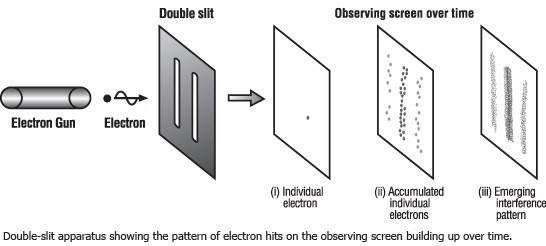
\includegraphics[keepaspectratio=true,width=.8\paperwidth]{.attachments/double-slit.jpeg}
    \caption{Image credit: ©2012 Perimeter Institute for Theoretical Physics, via https://www.perimeterinstitute.ca/research/research-areas/quantum-foundations/more-quantum-foundations.}
    \end{figure}
\end{frame}

%Start of slide
\begin{frame}{Quantum world if fascinating}{Particles behave like waves}
	\center
	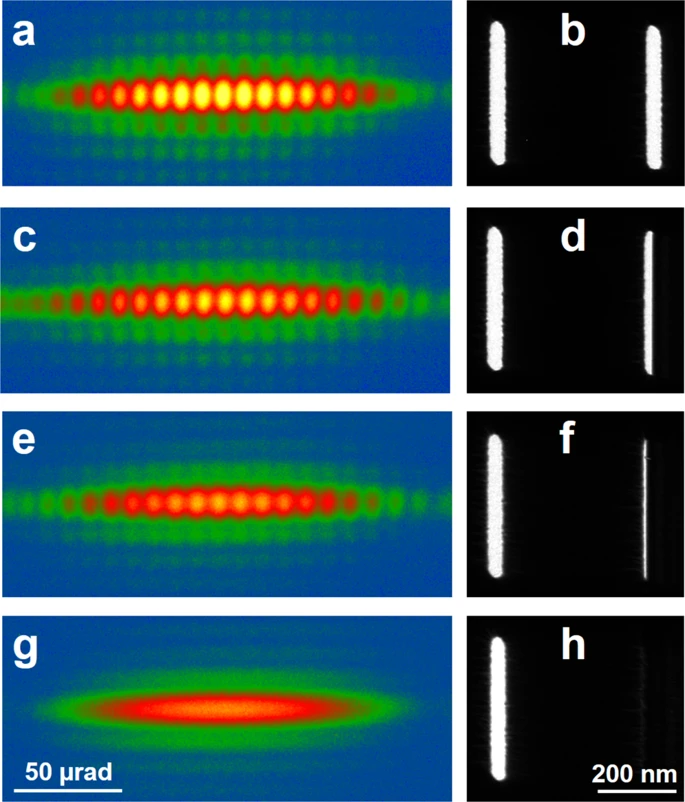
\includegraphics[keepaspectratio=true,width=.5\paperwidth]{.attachments/young.png}
\end{frame}

%Start of slide
\begin{frame}{Quantum world if fascinating}{Particles behave like waves}
    \justifying
    The state of a particle after passing through either one of the slits can be described as a \textit{wave} function (probability distribution) namely $\Psi = (\alpha_0 \psi_0 + \alpha_1 \psi_1)$ with $\{\alpha_0,\alpha_1\} \in \mathbb{C}$

    \center
	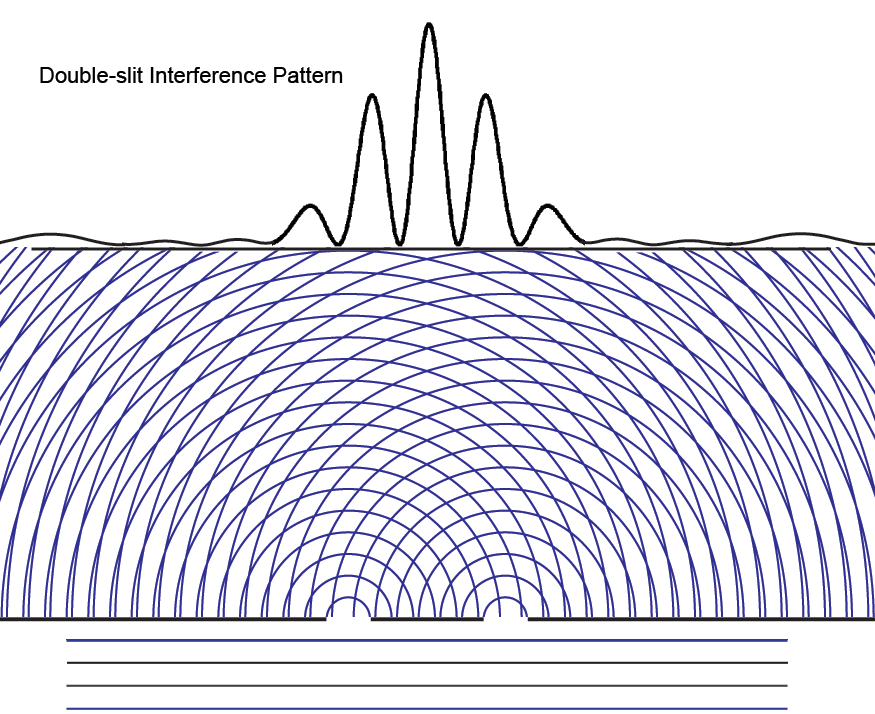
\includegraphics[keepaspectratio=true,width=.5\paperwidth]{.attachments/double-slit-distro.png}
\end{frame}


%Start of slide
\begin{frame}{Basic Unit of information: Bits}
	\justifying
	Traditional computation works with 0 and 1 as basic units of information. A physical realization of this is voltage from 0V to 5V
	\center
	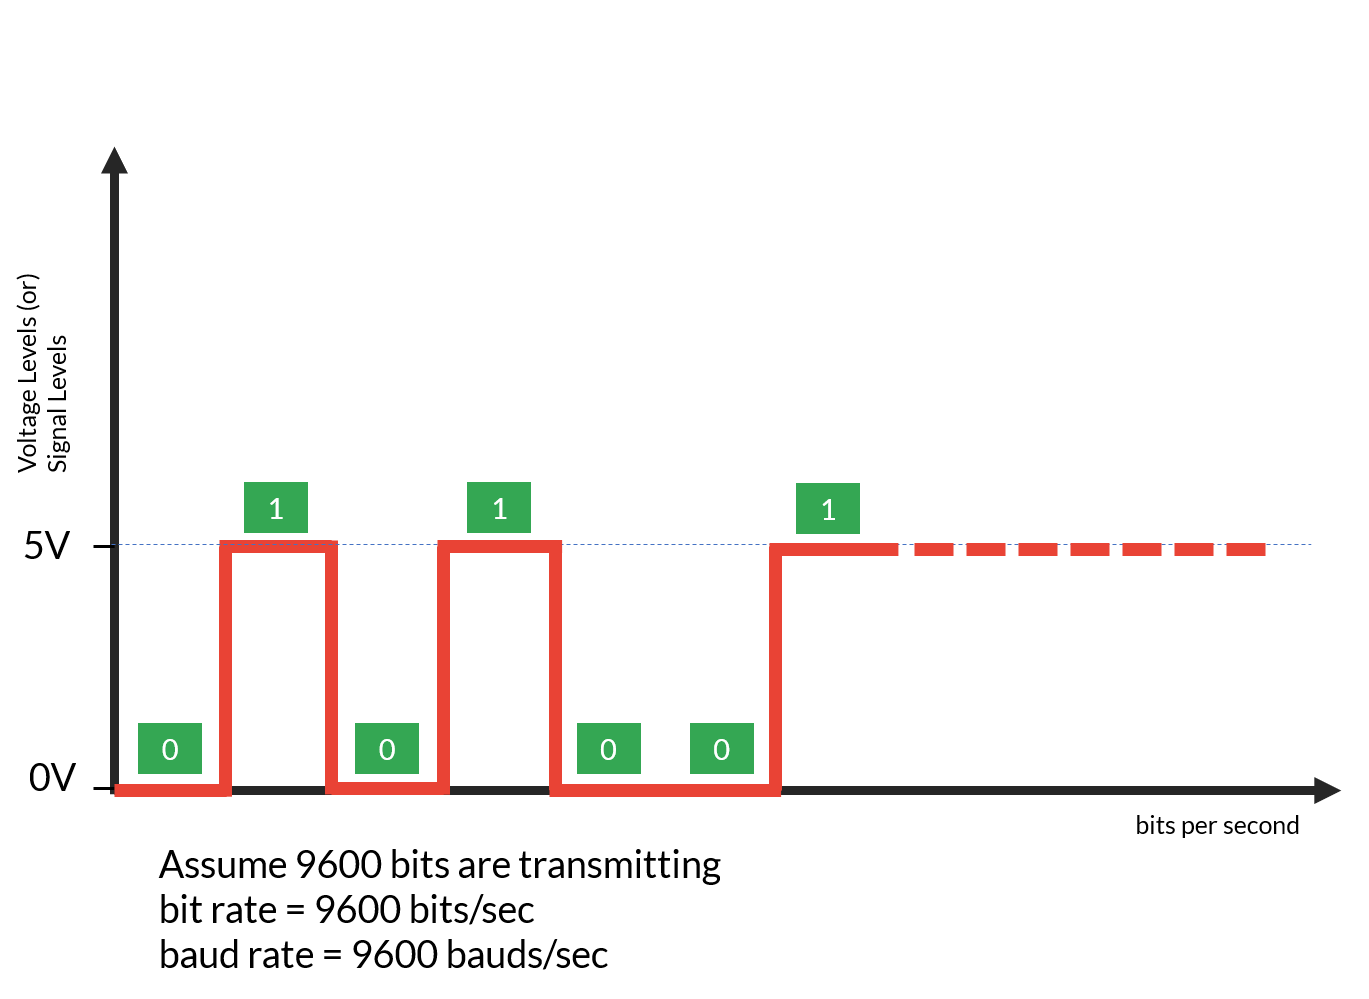
\includegraphics[keepaspectratio=true,width=.6\paperwidth]{.attachments/Bitrateequalbaudrate.png}
\end{frame}


%Start of slide
\begin{frame}{Basic Unit of information: Qubits}
	\justifying
	Quantum computation works with $\ket{0}$ and $\ket{1}$ as basic units of information. A physical realization of this would be a spin 1/2 particle.
	
	\center
	\includegraphics[keepaspectratio=true,width=.8\paperwidth]{.attachments/Qubit.png}
\end{frame}


%Start of slide
\begin{frame}{Computational basis states}
	\justifying
	Qubits can be in different states \textit{other} than $\ket{0}$ or $\ket{1}$. It is possible to form \textit{linear combinations} of states, called superpositions:
	$$\ket{\psi}= \alpha_0 \ket{0} + \alpha_1 \ket{1}$$
    The numbers $\alpha_0$ and $\alpha_1$ are complex numbers and ${|\alpha_0|}^2+|\alpha_1|^2=1$. 
    \newline
    \newline
Where $\ket{0}$ and $\ket{1}$ are vectors $\begin{pmatrix} 1 \\ 0 \end{pmatrix}$ and $\begin{pmatrix} 0 \\1 \end{pmatrix}$ in ${\mathbb{C}}^2$.
    \newline
    \newline
	A superposition state is a linear combination $ \psi =\alpha_0 \begin{pmatrix} 1 \\ 0 \end{pmatrix} + \alpha_1 \begin{pmatrix} 0 \\ 1 \end{pmatrix}$
\end{frame}

%Start of slide
\begin{frame}{Quantum NOT gate}
	\justifying
	Classical computer circuits consists of wires and logic gates. E.g. the NOT gate which has a truth table $0 \rightarrow 1$ and $1 \rightarrow 0$.
    \newline
    \newline
    The analogous quantum operation would take

    $$\alpha_0 \ket{0} + \alpha_1 \ket{1} $$

    to 

    $$\alpha_0 \ket{1} + \alpha_1 \ket{0} $$
    \newline
    \newline
    Since a quantum state can be represented as a vector, we are looking for a matrix such that:
    $$\mathrm{X} \begin{bmatrix} \alpha_0 \\ \alpha_1 \end{bmatrix}=\begin{bmatrix} \alpha_1 \\ \alpha_0 \end{bmatrix}$$ 
\end{frame}



\begin{frame}{Quantum Gates}
	\justifying
	Quantum gates are represented by matrices applied on our vectors (qubits). Are all matrices valid Quantum Gates?...no.
	\newline
    \newline
	Recall that  ${|\alpha_0|}^2+|\alpha_1|^2=1$ for a quantum state 
	$$\alpha_0 \ket{0} + \alpha_1 \ket{1}$$.
	This must also hold for 
	$$\alpha_0^{'}  \ket{0} + \alpha_1^{'} \ket{1}$$
	after the gate has acted. It turns out that the appropriate condition on the matrix representing the gate is tha the matrix $U$ be unitary. That is (with $U^{\dagger}$ is the adjoint of $U$)
	$$U^{\dagger}U=I$$

\end{frame}	

\begin{frame}{Quantum Gates}
	\justifying 
	In classical computers we only have one non-trivial gate for one bit (NOT gate). In the case of Quantum computers we have many!
	\newline
	\newline
	For example the NOT gate:
	$$\mathrm{X} \equiv \begin{bmatrix} 0 & 1 \\ 
										1 & 0 \end{bmatrix}$$
	The $Haddamard$ gate
	$$\mathrm{H} \equiv \frac{1}{\sqrt{2}}\begin{bmatrix} 1 & 1 \\ 
	1 & -1 \end{bmatrix}$$

\end{frame}

\begin{frame}{Bibliografía}
	\begin{itemize}
		\item What is bit rate and baud rate with examples – bytesofgigabytes.com. (2019). Retrieved 20 January 2020, from http://www.bytesofgigabytes.com/embedded/bit-rate-and-baud-rate/
		      \newline
		\item {Nielsen, M., \& Chuang, I. (2010). Quantum Computation and Quantum Information: 10th Anniversary Edition. Cambridge: Cambridge University Press. doi:10.1017/CBO9780511976667}
		      \newline
		\item {Gulde, S., Riebe, M., Lancaster, G. et al. Implementation of the Deutsch–Jozsa algorithm on an ion-trap quantum computer. Nature 421, 48–50 (2003) doi:10.1038/nature01336}
		\item Tavabi, A., Boothroyd, C., Yücelen, E., Frabboni, S., Gazzadi, G., Dunin-Borkowski, R., \& Pozzi, G. (2019). The Young-Feynman controlled double-slit electron interference experiment. Scientific Reports, 9(1). doi: 10.1038/s41598-019-43323-2
		\item $Collapse of the Wave Function. (2020). Retrieved 21 January 2020, from http://www.informationphilosopher.com/solutions/experiments/wave-function_collapse/$
	\end{itemize}
\end{frame}

\end {document}


